\documentclass[journal]{IEEEtran}
\usepackage[utf8]{inputenc}
\usepackage[T1]{fontenc}
\usepackage{mathtools}
\usepackage{amssymb}
\usepackage{amsmath}
% Use the journal template's consecutive equation numbering.
\DeclareMathOperator*{\argmax}{arg\,max}
\DeclareMathOperator*{\argmin}{arg\,min}
\DeclareMathOperator{\diag}{diag}
\usepackage{amsthm}
\usepackage{thmtools}
\newtheorem{theorem}{Theorem}[section]
\newtheorem{lemma}[theorem]{Lemma}
\newtheorem{corollary}[theorem]{Corollary}
\newtheorem{proposition}[theorem]{Proposition}
\theoremstyle{definition}
\newtheorem{definition}[theorem]{Definition}
\newtheorem{example}[theorem]{Example}
\theoremstyle{remark}
\newtheorem{remark}[theorem]{Remark}
\newtheorem*{note}{Note}
\usepackage{booktabs}
\usepackage{array}
\usepackage{multirow}
\usepackage{tabularx}
\usepackage{longtable}
\newcolumntype{C}[1]{>{\centering\arraybackslash}p{#1}}
\newcolumntype{L}[1]{>{\raggedright\arraybackslash}p{#1}}
\usepackage{tikz}
\usepackage{pgfplots}
\pgfplotsset{compat=1.18}
\usetikzlibrary{
  arrows.meta,
  positioning,
  shapes.geometric,
  shadows,
  fit,
  calc,
  matrix,
  shapes.misc
}
\tikzset{
  base/.style = {rectangle, rounded corners, draw=black, minimum width=2.5cm, minimum height=1cm, text centered, font=\sffamily},
  startstop/.style = {base, fill=red!20, drop shadow},
  process/.style = {base, fill=blue!20, drop shadow},
  decision/.style = {diamond, aspect=1.5, draw=black, fill=green!20, drop shadow, align=center},
  arrow/.style = {thick, -{Stealth[length=3mm]}},
  matrix_style/.style={matrix of nodes, row sep=0.5cm, column sep=0.5cm, nodes={anchor=center}},
  dashdot/.style={dash pattern=on 3pt off 3pt on 1pt off 3pt}
}
\usepackage{algorithm}
\usepackage{algorithmicx}
\usepackage{algpseudocode}
\algrenewcommand\algorithmicrequire{\textbf{Input:}}
\algrenewcommand\algorithmicensure{\textbf{Output:}}
\usepackage{graphicx}
\usepackage{adjustbox}
\usepackage{url}
\usepackage{xcolor}
\usepackage{cite}
\usepackage[hidelinks]{hyperref}
\hypersetup{pdftitle={Verified Localized Episodic Grounding for Network Analysis: A Controlled Mechanism Study}}
\usetikzlibrary{shapes.symbols}

\renewcommand{\dblfloatpagefraction}{0.7}
\setlength{\dblfloatsep}{10pt plus 2pt minus 2pt}
\usepackage{placeins}
\begin{document}
\title{Verified Localized Episodic Grounding for Network Analysis: A Controlled Mechanism Study}
% TODO: Supply verified author names, affiliations, corresponding email and ORCIDs.
\author{}
\maketitle
\begin{abstract}
Memory-augmented language models use historical evidence to support classification without parameter updates. Compressing that evidence into reusable explanations can simplify inference but may omit exceptions or introduce unsupported rules. Existing approaches emphasize episodic retrieval, local reflection with feedback, or global semantic consolidation. Their different abstraction units, correction signals and grounding strategies motivate controlled comparisons of evidence retention and reuse. We propose Verified Localized Episodic Grounding (VLEG), which checks each generated reflection against its labeled historical source. Within a bounded refinement budget, separate generator and verifier calls to the same model revise rejected candidates and admit the first accepted reflection. Hybrid inference retrieves admitted reflections together with their source records, retaining concrete evidence alongside local guidance. Five symbolic evaluations at 7B and 70B model scales examine memory strategies, grounding, refinement, overhead and explanation diagnostics, finding improved coverage and source-label agreement but mixed downstream benefits. Across five historical-memory seeds on 1,000 shared UNSW-NB15 test fingerprints, VLEG achieves Macro-F1 of $59.68\%$, compared with $42.66\%$ for unverified first reflections and $63.92\%$ for raw retrieval. Relative to raw retrieval, attack recall rises from $71.39\%$ to $77.74\%$ and false positive rate from $38.13\%$ to $48.78\%$, while the paired conditional 95\% interval for the Macro-F1 difference is $[-5.91,-2.53]$ percentage points. These findings separate successful source checking from reliable cross-episode explanation and establish no universal hybrid-memory advantage or production readiness. Historical symbolic runs still require corrected-parser reruns, and broader validation requires independent data, cross-episode checks and completed human explanation review.
\end{abstract}
\begin{IEEEkeywords}
Episodic memory, hallucination mitigation, large language models, network traffic analysis, verified memory consolidation
\end{IEEEkeywords}

\section{Introduction}
\subsection{Background and Motivation}
Large language models can use examples to support classification and analysis without parameter updates \cite{brown2020language,lewis2020retrieval}. For network analysis, historical flow records and incident summaries offer evidence for interpreting new observations. Their usefulness depends on retaining relevant conditions and exceptions while avoiding unsupported conclusions. Finite and imperfectly used context windows make the selection and organization of this evidence important \cite{an2024why,liu2024lost}.

Persistent-memory systems provide access to experience beyond the current prompt \cite{packer2023memgpt,wang2023longmem,wang2024memoryllm}. Raw records preserve detail, while reflections and summaries supply compact guidance. However, a summary can omit an exception or turn an incidental attribute into a general rule. This paper examines that trade-off using controlled symbolic tasks and a public-flow benchmark.

The memory-design problem is particularly visible when a model must relate a new observation to a small collection of labeled examples. Keeping every detail can preserve useful exceptions, but the model must still infer which differences matter. Compressing the same examples into natural-language rules changes that burden: inference can follow the stored guidance, yet the guidance may be less faithful than the underlying records. The design decision therefore concerns both what is retained and what evidence accompanies an abstraction when it is reused.

Source agreement and general validity are distinct requirements. A proposed explanation can correctly describe one record while asserting a condition that fails elsewhere. For example, an observed attribute may coincide with a label without being sufficient to determine it. Checking the explanation against that single record cannot resolve the distinction. A useful memory system must consequently be evaluated beyond successful storage: the resulting memory should support predictions on reserved queries, and its explanatory claims should be examined separately. This motivates measuring memory coverage, label consistency and downstream outcomes together rather than treating an admission rate as a complete measure of memory quality.

\subsection{Memory Research and Study Positioning}
Memory-augmented language models retain and reuse experience through episodic retrieval, local reflection, and semantic consolidation \cite{wu2025from,zhang2024survey}. These approaches differ in their abstraction unit, correction signal and inference evidence. Feedback-based agents already revise behavior using past experience \cite{shinn2023reflexion,wang2024voyager}; global hypothesis methods also generate and verify abstractions \cite{agarwal2026hypothesis,he2024idea}. Our focus is the narrower combination of per-episode admission checking and evidence--reflection pairing. We compare its outcomes against raw and abstract memory rather than assuming that local verification or hybrid context is universally superior.

The choice between these approaches depends on what must be preserved and how stored knowledge will be reused. Episodic retrieval retains concrete examples; reflection converts local experience into reusable guidance; semantic consolidation summarizes patterns across records. Hybrid inference combines an abstraction with retrieved evidence. Each can be useful under suitable conditions, and each introduces different failure modes when evidence is incomplete or an abstraction is applied outside its support.

The specific research question is whether checking a local reflection before admission improves later classification enough to justify its construction cost. A second question is whether pairing that reflection with its source is preferable to supplying either component alone. These questions require controlled comparisons: a change in retrieval quality must be distinguished from a change in displayed context, and the opportunity to revise must be distinguished from the decision to discard. The proposed study evaluates those distinctions and reports where expected benefits do not occur.

\subsection{Proposed VLEG Method}
We propose Verified Localized Episodic Grounding (VLEG) to check local abstractions before they enter memory while retaining the evidence from which they were derived. A generator proposes a local reflection from historical attributes, and a verifier checks it against the labeled source episode. Rejected candidates receive critique and can be revised within a maximum budget $K$; the first accepted candidate is stored with its source record. At inference, retrieved tuples provide both raw evidence and accepted reflections.

Generation and verification are separate calls to the same model. Target labels are withheld from inference. The admission check can expose contradictions with a source episode, but acceptance remains an imperfect model judgment: it does not establish causal validity or transfer to other episodes. These limits define the questions examined experimentally.

The consolidation procedure operates on labeled historical episodes rather than on the target query. A proposed reflection may summarize a local condition or heuristic. If the verifier rejects it, the critique becomes available to the next generation attempt. The iteration budget bounds the number of attempts; an episode whose proposals remain rejected is omitted from the admitted bank. This creates a practical trade-off between construction work and the amount of historical evidence retained for inference.

Each admitted tuple keeps the episode and its accepted reflection together, allowing the inference prompt to expose both. The method formulation retrieves tuples through semantic similarity and constructs hybrid context from the selected memories. Keeping the source visible provides evidence with which to assess the abstraction, although the reasoning model can still follow misleading guidance. The public-flow evaluation uses shared raw-feature retrieval to control example selection across local conditions; it tests consolidation and admission under that adaptation, not every component of reflection-driven retrieval.

The framework's intended contribution is thus an explicit, inspectable memory-admission procedure and a controlled evaluation of its consequences. The verifier does not access an independent population of episodes, and generator/verifier roles share model weights. Neither the stopping rule nor source consistency supplies a universal correctness guarantee. The resulting memory bank records which source supports each abstraction, while the explicit information-access boundaries make clear what an admission decision can establish.

\subsection{Experimental Evaluation}
We evaluate VLEG on symbolic tasks at 7B and 70B model scales and on a controlled public-flow benchmark. Comparisons vary memory construction, inference context and refinement budget, while tracking construction cost and reflection quality. Memory coverage and source-label agreement can improve without corresponding gains in explanation support or downstream classification.

On 1,000 shared UNSW-NB15 test fingerprints across five memory seeds, VLEG improves Macro-F1 over unverified first reflections by $17.02$ percentage points, but remains below raw retrieval: $59.68\%$ versus $63.92\%$. Higher attack recall accompanies more false alarms. We report these trade-offs, paired conditional uncertainty and costs, alongside the limits of repeated queries, historical-run provenance and incomplete human explanation review.

The symbolic evaluations provide a known oracle with controllable irrelevant attributes and withheld combinations. This setting lets us distinguish recovery of omitted evidence from improvements in the explanations themselves. It also exposes whether raw, abstract or hybrid context best supports withheld combinations, and whether additional revision attempts justify their construction cost. Public-flow records then test the same memory-design questions in a different domain. Seen-combination accuracy and masked-only accuracy are distinguished because they measure different forms of application and transfer. Historical symbolic numbers are linked to archived source versions, but corrected-parser reruns remain necessary where original verifier replies are unavailable.

The flow study adds prediction-level checkpoints, fixed source/model identifiers and paired uncertainty estimates. The VLEG-minus-raw Macro-F1 difference is $-4.24$ percentage points, with a conditional 95\% interval of $[-5.91,-2.53]$. Its admission coverage is $98.75\%$, yet 113 of 157 parseable admitted rules have contrary-label matches among other historical draws. These counterexamples do not constitute a human causal audit, but demonstrate why source agreement alone is insufficient. Construction costs and fixed-order latency limitations are reported alongside classification. Together, the evaluations establish a bounded account of verified local memory, including stronger label agreement, mixed transfer and a recall--false-alarm trade-off, rather than an unconditional performance advantage.

\subsection{Paper Organization}
The remainder of this paper moves from the memory-design choices motivating the study to the proposed framework and its empirical assessment. Section II reviews episodic retrieval, local reflection and semantic consolidation, clarifying the differences in evidence retention, feedback and inference context that guide our comparisons. Building on this discussion, Section III develops VLEG, explains its memory-consolidation and hybrid-inference phases, and specifies the verification loop, information-access boundaries and overall algorithm. Section IV then evaluates the framework through controlled symbolic comparisons and a public-flow benchmark. It examines memory strategies, grounding modalities, refinement budgets, construction costs and reflection quality, before discussing what the findings support and where the evidence remains limited. Finally, Section V brings together the principal conclusions and identifies the further validation needed for broader use of verified local memory.

\section{Related Work}
\subsection{Episodic Memory and Retrieval}
In-context learning uses demonstrations in the prompt to support task adaptation without parameter updates \cite{brown2020language}. Retrieval-augmented generation connects generation to external evidence retrieved for the current input \cite{lewis2020retrieval}. LongMem extends access to past context through a memory bank and retrieval mechanism \cite{wang2023longmem}. These approaches make historical evidence available without requiring every experience to be converted into a rule. Their memory contents and training procedures differ, so they should not be treated as interchangeable implementations of a single memory architecture.

Retrieval studies address demonstration selection \cite{zhang2022active,purohit2025sample} and effective context length \cite{an2024why}, complementing broader surveys of memory design \cite{wu2025from,zhang2024survey}. These questions concern which evidence reaches inference, independently of whether that evidence is subsequently summarized.

For labeled classification tasks, raw-example retrieval offers a direct control: each historical record retains its observed features and label. It can preserve exceptions that a compressed summary omits, but its usefulness depends on selecting relevant examples within a finite context budget. A retrieved example also does not establish that a neighboring target has the same label. Retrieval relevance, evidence coverage and prediction correctness therefore require separate evaluation.

Our raw-memory baseline follows this evidence-preserving principle. It provides labeled historical episodes at inference without reflection-generation calls. The symbolic experiments compare it with abstract and hybrid context, while the public-flow experiment shares label-free feature retrieval across conditions to control example selection. This adaptation isolates the supplied memory content more closely than a comparison that changes both retrieval and context construction. It remains a controlled classification baseline, rather than a reproduction of the full training and retrieval procedures of the cited systems.

\subsection{Local Reflection and Feedback}
MemoryBank stores, retrieves and updates information from past interactions \cite{zhong2024memorybank}. Generative agents combine an experience store with higher-level reflections \cite{park2023generative}, while Reflexion converts task feedback into verbal reflections retained for subsequent trials \cite{shinn2023reflexion}. These works show several ways to use experience beyond storing raw examples. They differ in what constitutes an episode, which feedback is available, when memories are updated and how stored text influences later behavior.

Related work also examines procedural skill acquisition \cite{wang2024voyager}, structured agent memory \cite{xu2025amem}, and timeline-based memory management \cite{kim2024towards}. Their different memory objectives motivate explicit controls for the classification setting studied here.

The distinction between feedback and verification is especially relevant here. Feedback can identify an unsuccessful action or prediction and motivate revision. A source-episode check instead asks whether a candidate explanation agrees with the observed record under a specified prompt. Neither mechanism, by itself, proves that the resulting explanation identifies the correct causal factors. A reflection may repair its label while retaining an unsupported threshold or treating an incidental attribute as a general condition.

VLEG studies a bounded per-episode admission procedure: generate a candidate, check it against the labeled source, revise rejected candidates, and store an accepted reflection with its evidence. Historical labels are available to the check, whereas target labels are excluded from inference. We distinguish an unverified first proposal from a feedback-based multi-attempt comparator; these provide different opportunities for correction. Both are controlled adaptations, not complete reproductions of published agent systems. The evaluation consequently separates admission coverage and source-label agreement from explanation support and downstream generalization.

\subsection{Semantic Consolidation and Hybrid Grounding}
Semantic consolidation compresses experience into hypotheses or summaries that guide subsequent reasoning. Hypothesis-Driven Reasoning iteratively generates and verifies hypotheses against episodic evidence, then combines hypotheses with retrieved episodes at inference \cite{agarwal2026hypothesis}. It provides a close comparison for the unit of abstraction: hypotheses induced across episodes versus VLEG's reflections attached to individual source records. Global hypotheses can express conditional relations; indeed, one background-conditioned rule represents our synthetic environment. Heterogeneity alone therefore does not imply that global abstraction must fail.

Inductive reasoning and hypothesis generation are studied in \cite{he2024idea,kim2022playgrounds,lee2024generating,qiu2024phenomenal,zhou2024hypothesis}; complementary work considers memory architectures \cite{kim2023machine,li2024memory,wang2025mirix} and iterative feedback or critique \cite{madaan2023selfrefine,gou2024critic}. We compare these research directions through abstraction scope, correction signals and inference evidence.

Hybrid grounding supplies both an abstraction and supporting examples. This retains access to concrete evidence, but can introduce conflicting guidance when the abstraction is inaccurate or applies too broadly. Its effectiveness depends on the content and applicability of the reflection, not merely the presence of both memory types. Comparing raw, abstract and hybrid context is necessary to identify these trade-offs.

VLEG's contribution is a controlled assessment of local admission checking and evidence--reflection pairing, including their limitations. The public-flow evaluation also includes raw retrieval restricted to admitted episodes, helping distinguish admission from reflection content. We report balanced classification, attack recall, false alarms and construction cost rather than inferring utility from memory coverage alone. These comparisons test when verified local memory is useful without assuming a universal advantage over direct retrieval or global consolidation.

\section{The Proposed Method}
\label{sec:vleg-methodology}
\subsection{Overview of Verified Localized Episodic Grounding (VLEG)}
VLEG stores a labeled historical episode with an accepted local reflection. The implementation distinguishes generation, checking and inference roles. The following formulation describes their information access and stopping behavior; it does not guarantee correctness of the verifier or general validity of an accepted rule.

Let $\mathcal{E}=\{e_1,\ldots,e_n\}$ be historical episodes whose labels are available during consolidation. A pure episodic memory stores those labeled episodes directly. The symbolic evaluations use scene tuples, while the public-flow evaluation uses UNSW-NB15 feature records from separate historical and test partitions. Write $e_i=(x_i,y_i)$, where $x_i$ denotes observed attributes and $y_i$ the historical label. The initial generator receives only $x_i$; the verifier receives $(x_i,y_i)$, and its critique can reveal $y_i$ during revision. Test labels are excluded from inference in either setting.

Conversely, global semantic consolidation \cite{agarwal2026hypothesis} attempts to distill $\mathcal{E}$ into a compact set of universal rules or hypotheses, $\mathcal{H}$. This can be modeled as finding a global hypothesis set that maximizes the likelihood of the observed episodes:
\begin{equation}
    \mathcal{H}^* = \arg\max_{\mathcal{H}} P(\mathcal{H} \mid e_1, e_2, \dots, e_n)
\end{equation}
A single conditional hypothesis can represent the contextual rule used here. In other datasets, a limited-length summary may omit important exceptions. This is a capacity and evidence question, not a consequence that follows from heterogeneity alone.

VLEG bridges this gap by shifting the abstraction target from the global distribution to the localized episode, while applying a model-based source-episode admission check. Rather than attempting to find a universal $\mathcal{H}^*$, VLEG constructs a memory bank consisting of verified episodic-semantic tuples:
\begin{equation}
    \mathcal{M}_{VLEG} = \left\{ (e_i, r_i^*) \mid e_i \in \mathcal{E}, \; \mathcal{V}(r_i^* \mid e_i) = 1 \right\}
\end{equation}
where $r_i^*$ is a localized semantic reflection (a detection rule or heuristic) derived specifically from episode $e_i$, and $\mathcal{V}(\cdot \mid e_i)$ is a strict verification function that returns $1$ when the implemented verifier accepts the candidate under its checking prompt; acceptance is a model judgment and can be wrong.

\begin{figure*}[!t]
\centering
\begin{adjustbox}{max width=\linewidth}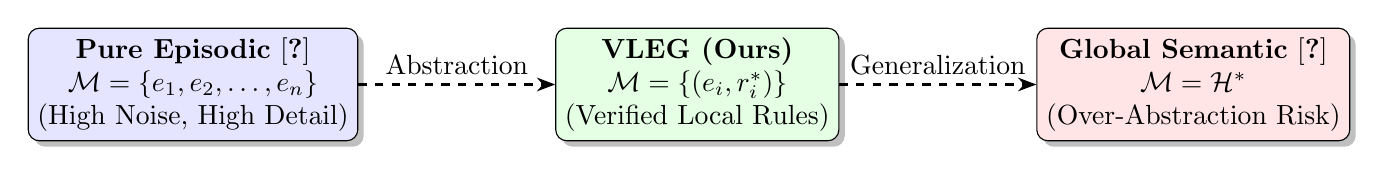
\begin{tikzpicture}[
    node distance=2cm and 2.5cm,
    box/.style={draw, rectangle, rounded corners, minimum width=3.5cm, minimum height=1.2cm, align=center, fill=gray!10, drop shadow},
    arrow/.style={-Stealth, thick}
]
% Nodes
\node[box, fill=blue!10] (episodic) {\textbf{Pure Episodic} \cite{brown2020language}\\$\mathcal{M} = \{e_1, e_2, \dots, e_n\}$\\(High Noise, High Detail)};
\node[box, fill=green!10, right=of episodic] (vleg) {\textbf{VLEG (Ours)}\\$\mathcal{M} = \{(e_i, r_i^*)\}$\\(Verified Local Rules)};
\node[box, fill=red!10, right=of vleg] (semantic) {\textbf{Global Semantic} \cite{agarwal2026hypothesis}\\$\mathcal{M} = \mathcal{H}^*$\\(Over-Abstraction Risk)};
% Arrows
\draw[arrow, dashed] (episodic) -- node[above] {Abstraction} (vleg);
\draw[arrow, dashed] (vleg) -- node[above] {Generalization} (semantic);
\end{tikzpicture}\end{adjustbox}
\caption{The theoretical positioning of VLEG within the memory abstraction spectrum. VLEG bridges the gap between pure episodic retention of raw traffic and global semantic consolidation by pairing raw episodes with accepted local abstractions.}
\label{fig:vleg_spectrum}
\end{figure*}
The stored tuple retains the source episode alongside its accepted reflection. This permits later comparison with the evidence, although the inference model may still follow an unsupported condition. The admission gate is only as reliable as the verifier for the specified error class.

\subsection{Framework Components: Generator, Verifier, and Memory Bank}
The implementation has a reflection generator, a verifier and a memory bank. Generation and checking use separate prompts and model calls. They use the same underlying model, so shared errors and dependent responses remain possible.

\subsubsection{The Reflection Generator ($\mathcal{G}_\theta$)}
The Reflection Generator is an LLM parameterized by $\theta$, tasked with distilling a high-dimensional raw traffic episode $e_i$ into a localized, natural language abstraction $r_i$. Formally, at iteration $j=0$, the generator samples an initial candidate reflection conditioned solely on the label-free attributes $x_i$:
\begin{equation}
    r_i^{(0)} \sim \mathcal{G}_\theta(\cdot \mid x_i)
\end{equation}
In subsequent iterations ($j > 0$), if the initial reflection is deemed invalid, the generator is conditioned on the raw episode, its previous candidate reflection $r_i^{(j-1)}$, and a natural language critique $c^{(j-1)}$ provided by the verifier:
\begin{equation}
    r_i^{(j)} \sim \mathcal{G}_\theta(\cdot \mid x_i, r_i^{(j-1)}, c^{(j-1)})
\end{equation}
The unverified single-step comparator stores its first proposal without checking. Feedback-based Reflexion \cite{shinn2023reflexion} is a different comparator: our latest symbolic adaptation uses bounded binary feedback and always stores a reflection. VLEG instead stores a candidate only after its source-episode check accepts it.

\subsubsection{The Strict Verifier ($\mathcal{V}_\phi$)}
The verifier checks the candidate against one labeled historical episode. It can reject a mismatched label, an invented attribute or an uncheckable claim. This role is distinct from generation, but the two calls are not statistically independent.

The verifier outputs a tuple consisting of a binary validity score $v^{(j)} \in \{0, 1\}$ and a diagnostic critique $c^{(j)}$:
\begin{equation}
    (v^{(j)}, c^{(j)}) = \mathcal{V}_\phi(e_i, r_i^{(j)})
\end{equation}
If $v^{(j)}=1$, the candidate passes the implemented admission check. If $v^{(j)}=0$, its critique is returned to the generator. Admission establishes only that this verifier accepted the reflection for this episode; it does not certify a universal rule or a lower false-positive rate than another system.

\subsubsection{The Hybrid Memory Bank ($\mathcal{M}$)}
Once a reflection successfully passes the verifier (i.e., $v^{(j)} = 1$), it is denoted as the verified reflection $r_i^*$. The Hybrid Memory Bank $\mathcal{M}$ stores the paired tuple of the raw episode and its verified abstraction:
\begin{equation}
    \mathcal{M} = \bigcup_{i=1}^{n} \left\{ (e_i, r_i^*) \mid \exists\,0\le j<K \text{ s.t. } \mathcal{V}_\phi(e_i, r_i^{(j)})_v = 1 \right\}
\end{equation}
Here $K$ is the maximum number of generation--verification attempts, indexed $j=0,\ldots,K-1$, including the initial proposal. The first accepted candidate is retained. If none is accepted, the episode is omitted from this bank; rejection alone does not establish that the episode is ambiguous or its proposed explanation false.

The memory bank supports retrieval of both source evidence and a local reflection. This is the representation used in the hybrid modality; raw-only and abstract-only inputs remove one of its components for comparison.

\begin{figure*}[!t]
\centering
\begin{adjustbox}{max width=\linewidth}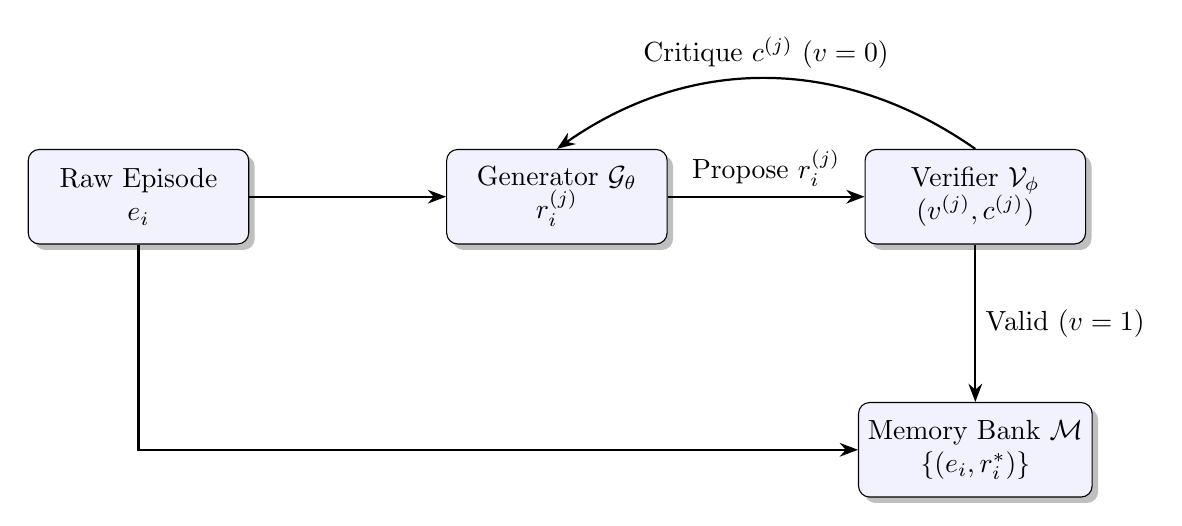
\begin{tikzpicture}[
    node distance=2cm and 2.5cm,
    box/.style={draw, rectangle, rounded corners, minimum width=2.8cm, minimum height=1.2cm, align=center, fill=blue!5, drop shadow},
    arrow/.style={-Stealth, thick}
]
% Nodes
\node[box] (episode) {Raw Episode\\$e_i$};
\node[box, right=of episode] (generator) {Generator $\mathcal{G}_\theta$\\$r_i^{(j)}$};
\node[box, right=of generator] (verifier) {Verifier $\mathcal{V}_\phi$\\$(v^{(j)}, c^{(j)})$};
\node[box, below=of verifier] (memory) {Memory Bank $\mathcal{M}$\\$\{(e_i, r_i^*)\}$};
% Arrows
\draw[arrow] (episode) -- (generator);
\draw[arrow] (generator) -- node[above] {Propose $r_i^{(j)}$} (verifier);
\draw[arrow] (verifier.north) to[bend right=35] node[above] {Critique $c^{(j)}$ ($v=0$)} (generator.north);
\draw[arrow] (verifier) -- node[right] {Valid ($v=1$)} (memory);
\draw[arrow] (episode.south) |- (memory.west);
\end{tikzpicture}\end{adjustbox}
\caption{Architectural flow of the VLEG framework components. Separate generator and verifier calls admit only candidates accepted by the implemented check to the Hybrid Memory Bank alongside their raw episodic counterparts.}
\label{fig:vleg_components}
\end{figure*}

\subsection{Learning Mechanism: Iterative Cyclic Refinement}
The refinement loop revises a rejected candidate using the verifier critique. It stops at the first accepted candidate or after $K$ attempts. Reaching the budget without acceptance discards the episode from this reflection memory.

Formally, let $e_i \in \mathcal{E}$ denote a raw, high-dimensional traffic episode. The refinement process is governed by two prompted roles using the same underlying model: the Reflection Generator $G_\theta$ and the Strict Verifier $V_\phi$. At the initial iteration ($j=0$), the generator produces a candidate reflection conditioned solely on the label-free attributes $x_i$:
\begin{equation}
    r_i^{(0)} \sim G_\theta(\cdot \mid x_i)
\end{equation}
Once a candidate reflection $r_i^{(j)}$ is generated, it is passed to the verifier $V_\phi$. The verifier returns a model-based admission decision using the labeled source $e_i$; its correctness and repeatability are not guaranteed. It outputs a tuple consisting of a binary validity score $v_i^{(j)} \in \{0, 1\}$ and a natural language critique $c_i^{(j)}$:
\begin{equation}
    (v_i^{(j)}, c_i^{(j)}) = V_\phi(e_i, r_i^{(j)})
    \label{eq:verifier}
\end{equation}
Note that $V_\phi$'s only argument besides the candidate reflection is the single episode $e_i$ it was generated from --- by construction it has no access to any other episode. This can expose a reflection that misstates $e_i$'s own attributes or label, but is not sufficient to determine whether an attribute the reflection treats as necessary is actually causally relevant across episodes versus merely true of this one instance. This defines a key boundary condition of the verifier, which we investigate empirically in the memory-quality assessment (Section~\ref{sec:exp5}).

If $v_i^{(j)} = 1$, the reflection is accepted by the implemented check, the loop terminates, and the verified reflection $r_i^* = r_i^{(j)}$ is committed to the memory bank. If $v_i^{(j)} = 0$, the check rejects the candidate, which can also occur for a malformed verifier response. The critique $c_i^{(j)}$ is then fed back into the generator to produce a refined reflection for the next iteration:
\begin{equation}
    r_i^{(j+1)} \sim G_\theta(\cdot \mid x_i, r_i^{(j)}, c_i^{(j)})
\end{equation}
This process stops at the first acceptance or after $K$ attempts. Exhausting the budget stores no tuple for that episode, reducing coverage without establishing a precision benefit.

\begin{figure*}[!t]
\centering
\begin{adjustbox}{max width=\linewidth}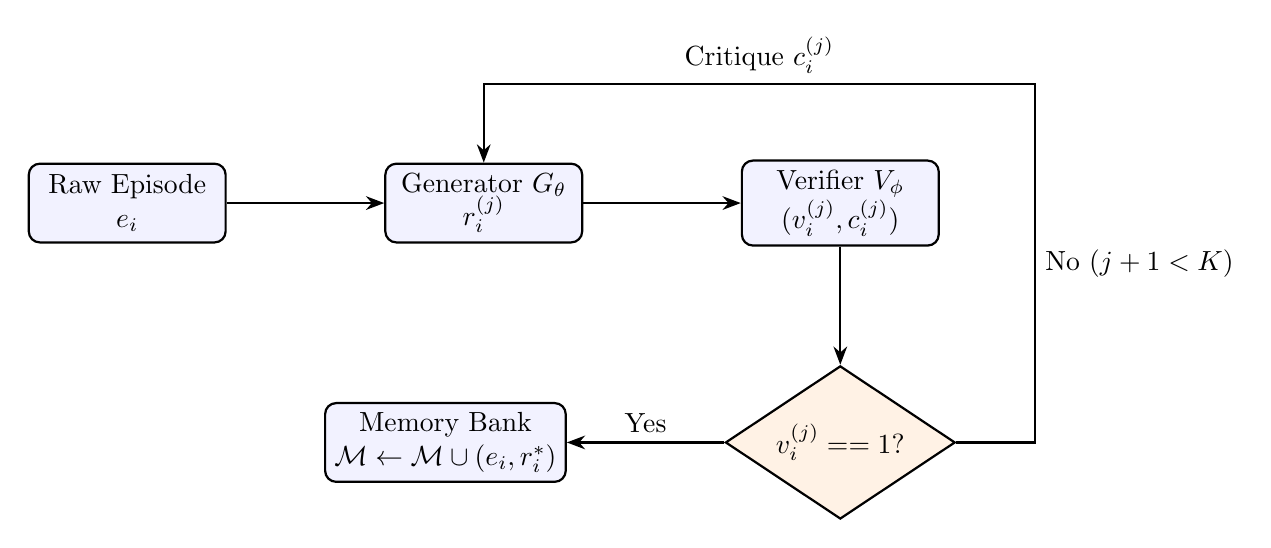
\begin{tikzpicture}[
    node distance=1.5cm and 2cm,
    box/.style={draw, rectangle, rounded corners, minimum width=2.5cm, minimum height=1cm, align=center, fill=blue!5, thick},
    decision/.style={draw, diamond, aspect=1.5, minimum width=2cm, align=center, fill=orange!10, thick},
    arrow/.style={-Stealth, thick}
]
% Nodes
\node[box] (episode) {Raw Episode\\$e_i$};
\node[box, right=of episode] (generator) {Generator $G_\theta$\\$r_i^{(j)}$};
\node[box, right=of generator] (verifier) {Verifier $V_\phi$\\$(v_i^{(j)}, c_i^{(j)})$};
\node[decision, below=of verifier] (check) {$v_i^{(j)} == 1$?};
\node[box, left=of check] (memory) {Memory Bank\\$\mathcal{M} \gets \mathcal{M} \cup (e_i, r_i^*)$};
% Arrows
\draw[arrow] (episode) -- (generator);
\draw[arrow] (generator) -- (verifier);
\draw[arrow] (verifier) -- (check);
\draw[arrow] (check) -- node[above] {Yes} (memory);
\draw[arrow] (check.east) -- ++(1,0)
    |- node[right, pos=0.25] {No ($j+1 < K$)}
       node[above, pos=0.75] {Critique $c_i^{(j)}$}
       ([yshift=1cm]generator.north)
    -- (generator.north);
%\draw[arrow] (check.east) -- ++(1,0) |- node[right, pos=0.25] {No ($j+1 < K$)} node[above, pos=0.75] {Critique $c_i^{(j)}$} (generator.north);
\end{tikzpicture}\end{adjustbox}
\caption{State transition diagram of the Iterative Cyclic Refinement mechanism. The loop stores the first candidate accepted by the verifier to the paired episodic--semantic memory bank.}
\label{fig:cyclic_refinement}
\end{figure*}
\begin{remark}[Scope of the admission check]
Let $A_j$ denote reaching attempt $j$, $E_j$ an erroneous candidate at that attempt, and $B_j$ its acceptance by the verifier. Using one-based attempt indices here, for $j=1,\ldots,K$, suppose
$\Pr(E_j\mid A_j)\leq p_h$ and
$\Pr(B_j\mid A_j,E_j)\leq p_v$ for a specified error class.
Since the loop stores the first accepted candidate,
\begin{equation}
\begin{aligned}
\Pr(\text{erroneous commitment})
&\leq \sum_{j=1}^{K}\Pr(A_j\cap E_j\cap B_j)\\
&\leq \min\{1,Kp_hp_v\}.
\end{aligned}
\end{equation}
This union bound needs no independence assumption. It does not imply that increasing $K$ reduces erroneous commitments, nor does it bound error conditional on admission. A geometric power of $p_v$ would require repeated acceptance checks on the same candidate, which the implemented loop does not perform. The probabilities are not estimated by the present experiments.
\end{remark}
A single labeled episode can expose a contradiction or a fabricated attribute, but cannot establish which attributes cause a label or whether a heuristic transfers to other episodes. The memory-quality assessment measures this distinction in the symbolic setting; public-flow explanations require additional cross-episode or human assessment.

\subsection{Inference Integration: Hybrid Episodic-Semantic Grounding}
Once the memory bank $\mathcal{M}$ has been populated with accepted tuples through the iterative cyclic refinement process, the system must effectively leverage this knowledge to solve a novel target task $T$ (e.g., classify a held-out flow or an unseen feature combination). Traditional retrieval-augmented generation (RAG) and standard in-context learning paradigms predominantly rely on episodic-only retrieval \cite{lewis2020retrieval, zhang2022active}, injecting raw, unstructured experiences directly into the context window. While this preserves high-fidelity details, it forces the reasoning module to perform ad-hoc abstraction at test time, which requires the inference model to infer useful relations from the retrieved examples. The present experiments do not establish that this requirement generally degrades performance.

To expose both representations at inference, VLEG uses a dual-pathway integration strategy termed \textit{Hybrid Episodic-Semantic Grounding}. This approach simultaneously injects the raw telemetry $e_i$ and its corresponding verified semantic rule $r_i^*$ into the context window, aligning with advanced memory integration paradigms that advocate for structured, multi-level memory representations \cite{wu2025from, zhang2024survey}. Our empirical evaluations further characterize the \emph{task- and scale-dependent boundary conditions} where hybrid grounding yields advantages versus when alternative grounding modalities perform comparably or better.

\subsubsection{Semantic-Driven Retrieval}
Given a novel target task $T$, the system must first retrieve the top-$k$ most relevant memory tuples. The symbolic VLEG formulation ranks admitted tuples by reflection embeddings. The public-flow adaptation instead ranks all historical records using label-free feature embeddings, then removes rejected records without replacement for VLEG and its admission control. These are distinct retrieval protocols, not interchangeable implementations.

Let $f_{\mathrm{emb}}(\cdot)$ denote a pre-trained dense embedding function. The relevance score $S(T, \mathcal{M}_i)$ for a given memory tuple $\mathcal{M}_i = (e_i, r_i^*)$ is computed using the cosine similarity between the embedding of the target task and the embedding of the verified reflection:
\begin{equation}
    S(T, \mathcal{M}_i) = \frac{f_{\mathrm{emb}}(T) \cdot f_{\mathrm{emb}}(r_i^*)}{\|f_{\mathrm{emb}}(T)\| \|f_{\mathrm{emb}}(r_i^*)\|}
\end{equation}
The system then selects the subset of $k$ tuples that maximize this similarity score:
\begin{equation}
    \mathcal{M}_{top} = \mathop{\arg\max}_{\mathcal{S} \subseteq \mathcal{M}, |\mathcal{S}|=\min(k,|\mathcal{M}|)} \sum_{(e_i, r_i^*) \in \mathcal{S}} S(T, (e_i, r_i^*))
\end{equation}

\subsubsection{Hybrid Prompt Formulation}
After retrieving $\mathcal{M}_{top}$, the inference module constructs a hybrid context window. The fundamental premise of hybrid grounding is that the verified reflection $r_i^*$ provides proposed local guidance, while the labeled source episode $e_i$ provides the observed evidence. Neither component is a validated causal explanation. This permits comparison with the source evidence, but does not guarantee that unsupported generalization is avoided.

The final inference prompt $P$ is constructed by concatenating the target task $T$ with the retrieved hybrid tuples, separated by structural delimiters:
\begin{equation}
\begin{aligned}
    Q_i &= \big[\text{Episode: }e_i \oplus \text{Verified Rule: }r_i^*\big],\\
    P &= \text{PromptBuilder}\Bigl(
    \bigoplus_{(e_i,r_i^*)\in\mathcal{M}_{top}} Q_i
    \oplus \text{Target: }T\Bigr).
\end{aligned}
\end{equation}
where $\oplus$ denotes the sequence concatenation operator. The reasoning LLM, parameterized by $\psi$, then generates the final prediction $\hat{y}$ conditioned on this hybrid prompt:
\begin{equation}
    \hat{y} = \text{LLM}_\psi(P)
\end{equation}

Hybrid context provides a reflection and its source evidence. Its benefit depends on whether the reflection guides the model toward relevant attributes or anchors it on a misleading condition. The grounding-modality ablation compares hybrid, raw-only and abstract-only inputs under shared retrieval.

\subsection{Final Algorithm and Execution Flow}
The Verified Localized Episodic Grounding (VLEG) framework synthesizes the previously defined components---the Reflection Generator $G_\theta$, the Strict Verifier $V_\phi$, and the Hybrid Inference Module $I_\psi$---into a cohesive, end-to-end execution pipeline. This pipeline systematically bridges the gap between raw episodic retention \cite{brown2020language} and abstract semantic reasoning \cite{agarwal2026hypothesis} by ensuring that only accepted local heuristics are utilized during downstream inference.

The execution flow of VLEG is formally divided into two distinct phases: \textbf{Phase 1: Memory Consolidation} and \textbf{Phase 2: Hybrid Inference}.

During Phase 1, the system ingests a stream of raw, high-dimensional traffic episodes $\mathcal{E} = \{e_1, e_2, \dots, e_n\}$. For each episode $e_i$, the Generator $G_\theta$ proposes $r_i^{(0)}$ from label-free attributes $x_i$. The Verifier $V_\phi$ then evaluates this candidate strictly against the grounding episode $e_i$, outputting a binary validity flag $v \in \{0, 1\}$ and a natural language critique $c$. If $v = 0$ (a rejected or unparseable check), the critique $c$ is fed back into $G_\theta$ to produce a refined reflection $r_i^{(1)}$. This iterative cyclic refinement continues until the reflection is validated ($v=1$) or a predefined maximum iteration limit $K$ is reached. If validated, the tuple $(e_i, r_i^*)$ is committed to the Memory Bank $\mathcal{M}$. The gate excludes rejected candidates from memory, but can retain an erroneous candidate if the verifier accepts it. This differs from unconditional first-proposal storage and from feedback-based reflection \cite{shinn2023reflexion}.

During Phase 2, the system is presented with a novel target task $T$. A Retriever $R$ computes the cosine similarity between the task embedding and the stored memory tuples, extracting the top-$k$ most relevant memories $\mathcal{M}_{top} \subset \mathcal{M}$. The Inference Module $I_\psi$ is then prompted using Hybrid Episodic-Semantic Grounding, receiving both the raw episodes and their verified reflections to generate the final output. This dual-pathway integration aligns with advanced memory paradigms \cite{wu2025from}, making both representations available for the evaluated inference conditions.

The complete step-by-step procedure is formalized in Algorithm \ref{alg:vleg_final}.

\begin{algorithm}[!t]
\caption{Verified Localized Episodic Grounding (VLEG)}
\label{alg:vleg_final}
\small
\begin{algorithmic}[1]
\Require Episodes $\mathcal{E}$, target $T$, max attempts $K$
\Statex Retrieval count $k$, retriever $R$
\State Initialize Memory Bank $\mathcal{M} \gets \emptyset$
\State \textbf{// Phase 1: Memory Consolidation}
\For{each $e_i \in \mathcal{E}$}
    \State $j \gets 0$
    \State $(r,c) \gets (\emptyset,\emptyset)$
        \Statex $\triangleright$ \textit{Previous candidate and critique}
    \State $v \gets 0$
        \Statex $\triangleright$ \textit{Initialize validity flag to Invalid}
    \While{$v = 0$ \textbf{and} $j < K$}
        \State $r_i^{(j)} \gets G_\theta(x_i, r, c)$
        \Statex $\triangleright$ \textit{Generate or refine reflection}
        \State $(v, c) \gets V_\phi(e_i, r_i^{(j)})$
        \Statex $\triangleright$ \textit{Check reflection against labeled source}
        \State $r \gets r_i^{(j)}$; $j \gets j + 1$
    \EndWhile
    \If{$v = 1$}
        \State $\mathcal{M} \gets \mathcal{M} \cup \{(e_i, r_i^{(j-1)})\}$
        \Statex $\triangleright$ \textit{Store verified tuple}
    \EndIf
\EndFor
\State \textbf{// Phase 2: Hybrid Inference}
\State $\mathcal{M}_{top} \gets R(\mathcal{M}, T, k)$
        \Statex $\triangleright$ \textit{Retrieve top-$k$ relevant tuples}
\State $\text{Context} \gets \text{PromptBuilder}(\mathcal{M}_{top},T)$
        \Statex $\triangleright$ \textit{Construct hybrid prompt}
\State $\text{Output} \gets I_\psi(\text{Context})$
        \Statex $\triangleright$ \textit{Generate final reasoning answer}
\State \Return $\text{Output}$
\end{algorithmic}
\end{algorithm}



The admission gate prevents storage when the verifier rejects a candidate. Its practical reliability depends on the verifier and the error class being checked. Retaining raw evidence permits downstream comparison with a reflection, but does not ensure that the model performs that comparison correctly.


\section{Experiments}

\subsection{Experimental Settings}
The symbolic evaluations use synthetic scenes with shape, color, texture, background and a deterministic size distractor. On white backgrounds, ANOMALY requires a red circle; black backgrounds invert this rule. Texture and size are noncausal. Level 1 contains eight white-background combinations; Level 2 contains sixteen across both backgrounds. Both evaluate combinations used to form memory. Level 3 withholds four from memory and tests all sixteen; masked-only accuracy measures withheld-combination generalization. Seeds change the withheld subset, not the underlying population.

Reported symbolic runs use Qwen2.5-7B-Instruct or Llama-3.3-70B-Instruct, nomic-embed-text embeddings and temperature $0$. Generator and verifier are separate calls to the same model. Initial generation excludes historical labels; verification receives labeled sources, and later attempts can receive labels through supervised critique. Target labels are reserved for scoring. We vary consolidation, grounding modality and $K\in\{1,2,3,5\}$, measuring accuracy, memory coverage, label consistency, attribution flags and construction tokens. The grounding-modality ablation shares retrieval across modalities. First-proposal reflections, feedback-based Reflexion and global hypotheses are controlled adaptations; their implementation differences are identified below.

The 7B and latest 70B archives have been reconciled, but lack original verifier replies and exact model digests. They precede strict boolean-parser repairs and were not rerun. Cross-scale comparisons also change model family and cannot isolate parameter count. Repeated queries across seeds are not independent samples, and temperature $0$ does not guarantee identical outputs. The public-flow benchmark separately specifies the public-flow data, frozen model versions, split, metrics and runtime costs.

\subsection{Controlled Memory-Strategy Comparison}
\label{sec:exp1}

We compare VLEG, global-hypothesis consolidation, unverified single-step reflection, and raw in-context retrieval on the three symbolic task levels. The comparisons characterize this small environment and these adaptations; they do not establish superiority over published systems on their original benchmarks.

Within each model-scale comparison the same underlying model and temperature are used. VLEG uses $K=3$. Level 1 has eight queries and Level 2 sixteen. Level 3 is pooled over three masking seeds, giving 48 evaluations of sixteen recurring combinations. Repeat runs matched reported accuracies in the checked conditions, which is an empirical repeatability observation rather than a determinism guarantee.

The reported 7B accuracies are ICL $100.0\%$, $93.8\%$ and $87.5\%$ at Levels 1--3, versus VLEG $75.0\%$, $87.5\%$ and $75.0\%$. Global-hypothesis consolidation recovers the uniform-background rule at Level 1 ($100.0\%$), but has pooled accuracy $70.8\%$ at Level 3. The historical single-step reflection comparator scores $25.0\%$, $50.0\%$ and $50.0\%$; the inspected first proposals predominantly state ANOMALY. Its aggregate accuracy tracks the anomaly base rate, although individual Level-3 seeds differ. These values describe the historical adaptation, not the changed multi-attempt feedback baseline now present in the repository.

\begin{figure}[!t]
    \centering
    \begin{adjustbox}{max width=\linewidth}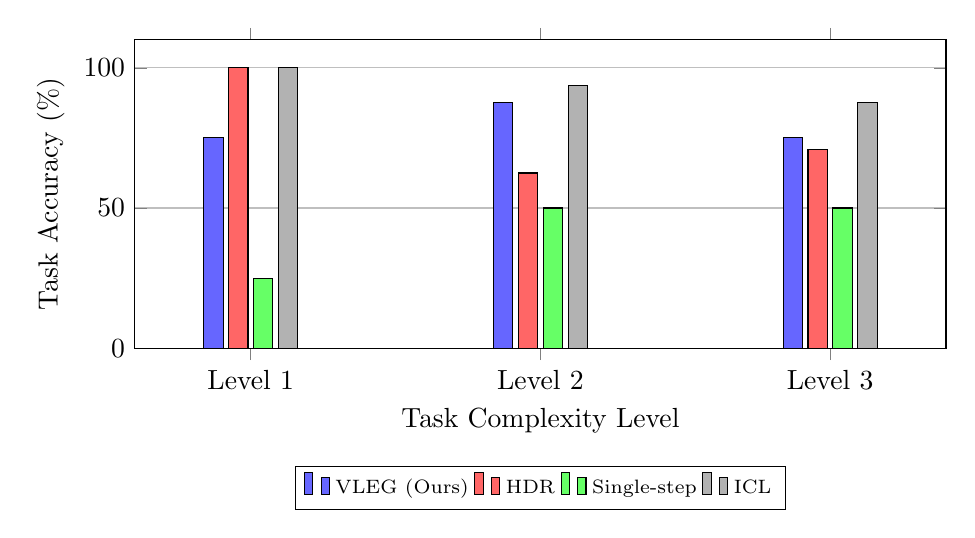
\begin{tikzpicture}
        \begin{axis}[
            ybar,
            bar width=7pt,
            width=0.98\linewidth,
            height=5.5cm,
            enlarge x limits=0.2,
            legend style={at={(0.5,-0.38)}, anchor=north, legend columns=-1, font=\scriptsize},
            ylabel={Task Accuracy (\%)},
            xlabel={Task Complexity Level},
            symbolic x coords={Level 1, Level 2, Level 3},
            xtick=data,
            ymin=0, ymax=110,
            grid=major,
            ymajorgrids=true,
            xmajorgrids=false,
        ]

        % VLEG
        \addplot[fill=blue!60] coordinates {(Level 1, 75.0) (Level 2, 87.5) (Level 3, 75.0)};
        \addlegendentry{VLEG (Ours)}

        % HDR
        \addplot[fill=red!60] coordinates {(Level 1, 100.0) (Level 2, 62.5) (Level 3, 70.8)};
        \addlegendentry{HDR}

        % Single-step
        \addplot[fill=green!60] coordinates {(Level 1, 25.0) (Level 2, 50.0) (Level 3, 50.0)};
        \addlegendentry{Single-step}

        % ICL
        \addplot[fill=gray!60] coordinates {(Level 1, 100.0) (Level 2, 93.8) (Level 3, 87.5)};
        \addlegendentry{ICL}

        \end{axis}
    \end{tikzpicture}\end{adjustbox}
    \caption{Measured Task Accuracy (\%) across three levels of task complexity (reduced-order reimplementation, Qwen2.5-7B-Instruct; Level 3 pooled across 3 masking seeds, $n=48$). ICL leads at every level; HDR is bimodal (perfect at Level 1's non-conditional rule, weak once the rule becomes background-conditional); Single-step tracks each level's ANOMALY base rate rather than discriminating between scenes.}
    \label{fig:exp1_results}
\end{figure}

At 7B, raw retrieval performs best in this environment. This limits the evidence for an advantage from consolidation at that scale. The grounding-modality ablation isolates grounding content more directly, and the limitations below explain why this globally expressible oracle does not establish a general weakness of global consolidation.

The reported 70B check evaluates Levels 1 and 2 once each and Level 3 across three masking seeds. The latest archived, feedback-baseline revision gives Level-3 pooled accuracies of VLEG $91.67\%$ (44/48), raw retrieval $89.58\%$ (43/48), global hypothesis $83.33\%$ (40/48), and feedback-based Reflexion $81.25\%$ (39/48). VLEG exceeds raw retrieval in two seeds but is lower in the third. These replace the earlier $93.75\%$ VLEG and single-step-baseline numbers; the feedback-based comparator is not the same condition as the 7B first-proposal comparator. This reverses the descriptive ordering at 7B. Because the model family also changes and the evaluation population is small, the difference should not be attributed to parameter count alone.

\subsection{Component Isolation (Grounding Modality Ablation)}
\label{sec:exp2}

This ablation compares hybrid, abstract-only and raw-only grounding while keeping retrieval fixed. Hybrid inference receives each retrieved episode $e_i$ and its accepted reflection $r_i^*$; abstract-only receives the reflection; raw-only receives the episode, following the example-based principle of ICL \cite{brown2020language}. All conditions retrieve the same top-$k$ tuples using reflection-embedding similarity. Thus the comparison changes displayed content rather than example selection, although it remains conditional on the admitted memory bank.

At 7B, Figure~\ref{fig:exp2_ablation} shows that hybrid grounding leads on Level 2: $87.5\%$ versus $81.2\%$ for both alternatives. On Level 3, five masking seeds give overall accuracies of hybrid $73.8\%$, abstract-only $78.8\%$ and raw-only $75.0\%$ ($n=80$ recurring evaluations). Masked-only accuracies are $60.0\%$, $70.0\%$ and $70.0\%$ ($n=20$). Hybrid does not outperform both alternatives in any Level-3 seed. Abstract-only therefore exceeds hybrid by $5.0$ percentage points overall and $10.0$ points on withheld combinations.

\begin{figure}[!t]
    \centering
    \begin{adjustbox}{max width=\linewidth}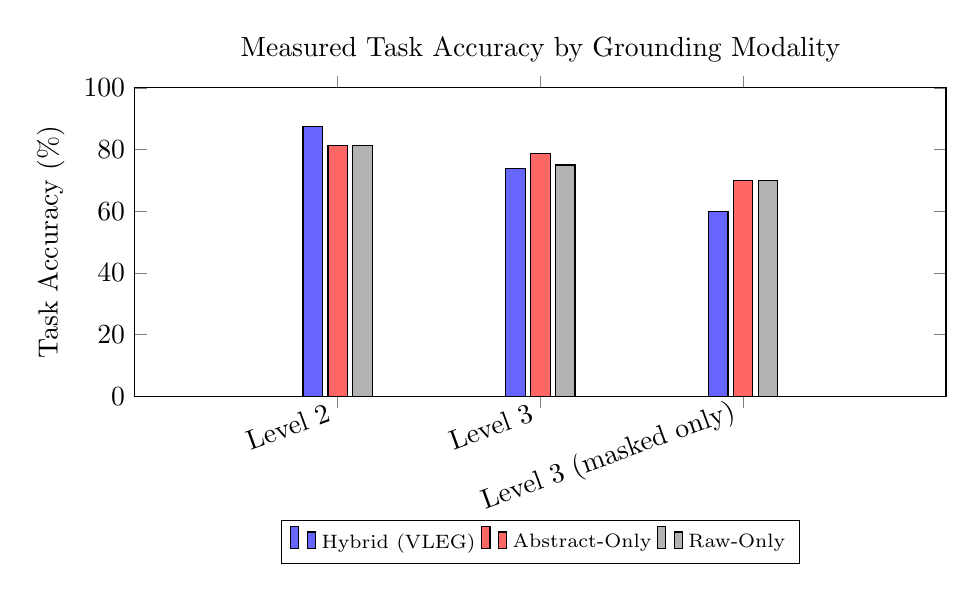
\begin{tikzpicture}
        \begin{axis}[
            ybar=2pt,
            bar width=7pt,
            width=0.98\linewidth,
            height=5.5cm,
            enlarge x limits=0.5,
            ylabel={Task Accuracy (\%)},
            ymin=0, ymax=100,
            symbolic x coords={Level 2, Level 3, Level 3 (masked only)},
            xtick=data,
            x tick label style={rotate=20, anchor=east},
            legend style={at={(0.5,-0.4)}, anchor=north, legend columns=-1, font=\scriptsize},
            title={Measured Task Accuracy by Grounding Modality}
        ]

        % Hybrid Grounding
        \addplot[fill=blue!60] coordinates {(Level 2, 87.5) (Level 3, 73.8) (Level 3 (masked only), 60.0)};
        \addlegendentry{Hybrid (VLEG)}

        % Abstract-Only Grounding
        \addplot[fill=red!60] coordinates {(Level 2, 81.2) (Level 3, 78.8) (Level 3 (masked only), 70.0)};
        \addlegendentry{Abstract-Only}

        % Raw-Only Grounding
        \addplot[fill=gray!60] coordinates {(Level 2, 81.2) (Level 3, 75.0) (Level 3 (masked only), 70.0)};
        \addlegendentry{Raw-Only}

        \end{axis}
    \end{tikzpicture}\end{adjustbox}
    \caption{Measured Task Accuracy across grounding modalities (reduced-order reimplementation, Qwen2.5-7B-Instruct). Level 3 figures are pooled across 5 masking seeds ($n=80$ overall, $n=20$ for the masked-only subset). Hybrid Grounding wins on Level 2 but is the worst condition on Level 3, especially on the masked combinations it was intended to help with --- the opposite of the original hypothesis.}
    \label{fig:exp2_ablation}
\end{figure}

The 70B comparison uses the same five masks. Hybrid and raw-only tie at $95.0\%$ overall, while abstract-only reaches $91.25\%$. On masked combinations, abstract-only remains higher at $85.0\%$, versus $80.0\%$ for both alternatives. Its per-seed masked accuracies are $100\%$, $75\%$, $50\%$, $100\%$ and $100\%$, illustrating the variability behind the pooled advantage. The overall 7B ordering consequently reverses, while the masked-only direction persists with a smaller gap.

These results separate overall performance from withheld-combination transfer. Raw evidence alongside a reflection does not guarantee a benefit: a reflection may add useful guidance or emphasize an unsupported condition. The memory-quality assessment in Section~\ref{sec:exp5} identifies irrelevant-attribute references, making misleading guidance a plausible explanation, but this ablation does not establish a causal anchoring mechanism. Because retrieval uses accepted-reflection embeddings, raw-only here also differs from direct raw-episode retrieval in Section~\ref{sec:exp1}. Conclusions are restricted to the controlled memory bank, model families and small recurring symbolic population; they do not establish a generally necessary or superior grounding modality.

\subsection{Iterative Refinement Ablation}
\label{sec:exp3}

The refinement ablation tests whether a larger revision budget recovers rejected episodes and changes downstream accuracy. Both $K=1$ and $K=3$ use the same generator, verifier and hybrid inference. At $K=1$, a rejected first proposal discards the episode; at $K=3$, critique permits further attempts before discard. This is a budget comparison, not verified versus unverified reflection: both conditions perform verification, and both stop at the first accepted candidate.

Across five 7B masking seeds, $K=3$ achieves $75.0\%$ overall accuracy ($60/80$), compared with $63.75\%$ ($51/80$) at $K=1$, an $11.25$-percentage-point increase. Masked-only accuracy rises from $50.0\%$ ($10/20$) to $60.0\%$ ($12/20$). The masked-only difference is zero in three seeds and positive in two. The pooled overall gain therefore does not imply that every memory draw improves transfer to withheld combinations. These are repeated evaluations of the same sixteen-element population under different masks, not eighty independent scenes.

The principal observed change is memory coverage. First-attempt verification retains approximately $42$--$58\%$ of historical episodes across seeds, whereas $K=3$ retains $83$--$100\%$. Rejection critique can reveal the correct historical label, allowing a revised candidate to agree with its source. Additional attempts consequently recover examples that the smaller budget would omit. The improvement is consistent with this coverage pathway; it is not evidence that each recovered explanation identifies the true causal attributes more reliably.

The archived 70B comparison reports a mean overall gain of $26.2$ percentage points, with sample standard deviation $8.1$ across the same five masks. All twelve historical episodes are admitted at $K=3$ in every seed. This demonstrates a larger descriptive budget effect in that model configuration, but the model family also changes, and the two scales cannot isolate parameter count. Neither the pooled gain nor full admission proves reliable generalization outside the specified symbolic oracle.

The comparison also clarifies what refinement can and cannot change. Increasing $K$ changes the opportunity to revise and the resulting evidence available at inference; it does not add new source observations or independently validate a generalized rule. Coverage recovery and explanation quality should therefore be assessed separately, as in Section~\ref{sec:exp5}. An accepted reflection can match a historical label while retaining a spurious condition that misguides a later query.

The results support bounded refinement as a means of reducing rejection-induced memory loss in this setting. They do not justify increasing the budget without considering cost or assuming a universal optimum. Section~\ref{sec:exp4} examines that trade-off across intermediate and larger ceilings. Missing original verifier replies in the historical archive also prevent quantifying the effect of the later strict-parser repair on these runs.

\subsection{Parameter Sensitivity and Overhead Analysis}
\label{sec:exp4}

We vary the maximum refinement budget over $K\in\{1,2,3,5\}$ and measure symbolic accuracy and construction prompt-plus-completion tokens per historical episode. At $K=1$, verification still occurs, but a rejected proposal cannot be revised. Level 2 uses a fixed population; Level 3 varies the withheld subset across three masking seeds. This sweep tests whether additional attempts change memory coverage enough to justify their cost.

\begin{figure}[!t]
    \centering
    \begin{adjustbox}{max width=\linewidth}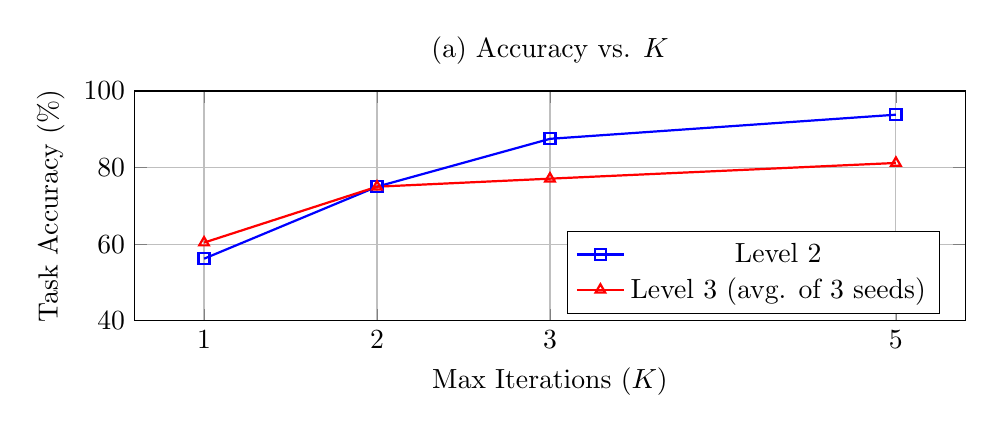
\begin{tikzpicture}
        \begin{axis}[
            width=\linewidth,
            height=4.5cm,
            xlabel={Max Iterations ($K$)},
            ylabel={Task Accuracy (\%)},
            ymin=40, ymax=100,
            xtick={1,2,3,5},
            grid=major,
            legend pos=south east,
            title={(a) Accuracy vs. $K$}
        ]
        \addplot[color=blue, mark=square, thick] coordinates {(1, 56.2) (2, 75.0) (3, 87.5) (5, 93.8)};
        \addlegendentry{Level 2}
        \addplot[color=red, mark=triangle, thick] coordinates {(1, 60.4) (2, 75.0) (3, 77.1) (5, 81.2)};
        \addlegendentry{Level 3 (avg. of 3 seeds)}
        \end{axis}
    \end{tikzpicture}\end{adjustbox}
    \par\vspace{0.5cm}
    \begin{adjustbox}{max width=\linewidth}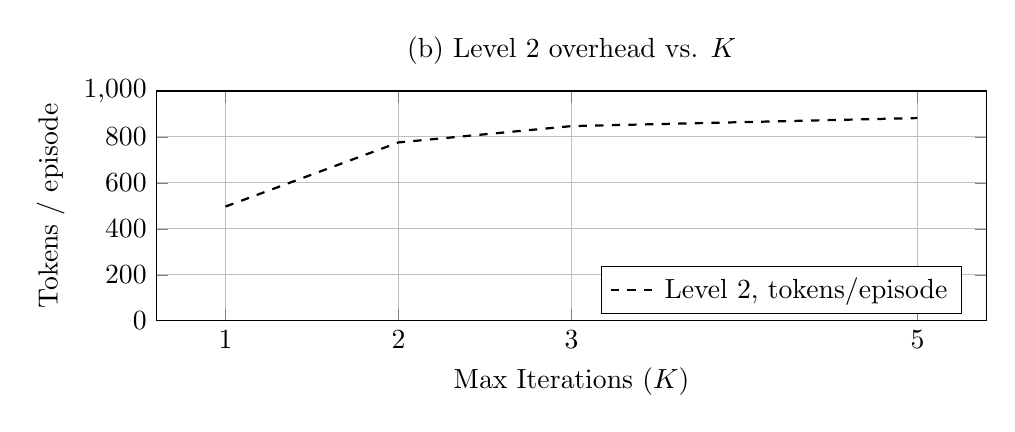
\begin{tikzpicture}
        \begin{axis}[
            width=\linewidth,
            height=4.5cm,
            xlabel={Max Iterations ($K$)},
            ylabel={Tokens / episode},
            ymin=0, ymax=1000,
            xtick={1,2,3,5},
            grid=major,
            legend pos=south east,
            title={(b) Level 2 overhead vs. $K$}
        ]
        \addplot[color=black, mark=circle, thick, dashed] coordinates {(1, 497) (2, 776) (3, 847) (5, 882)};
        \addlegendentry{Level 2, tokens/episode}
        \end{axis}
    \end{tikzpicture}\end{adjustbox}
    \caption{Measured parameter sensitivity of the maximum refinement iterations $K$ (reduced-order reimplementation, Qwen2.5-7B-Instruct). (a) Task Accuracy does \emph{not} plateau at $K=3$: Level 2 (a single run whose accuracy matched on repeat) keeps improving through $K=5$; Level 3 (averaged over 3 masking seeds) plateaus in only 1 of 3 seeds individually. (b) Token overhead per consolidated episode is concave, not linear: most of the cost increase happens between $K{=}1$ and $K{=}2$, with sharply diminishing marginal cost for extending the budget further, since only a minority of episodes ever use the additional iterations.}
    \label{fig:exp4_sensitivity}
\end{figure}

Figure~\ref{fig:exp4_sensitivity} shows no reliable 7B plateau at $K=3$. Level-2 accuracy rises from $87.5\%$ at $K=3$ to $93.8\%$ at $K=5$. In Level 3, only seed 42 has identical bank composition, tokens and accuracy at those budgets; the other masks do not reproduce that exact plateau. A budget sufficient for one mask can therefore remain insufficient for another. The figure's accuracy panel pools Level-3 seeds, while its token panel reports the Level-2 run.

Construction overhead grows less than linearly over the measured ceilings. Level-2 cost increases by approximately 279 tokens per episode from $K=1$ to $K=2$, 71 from $K=2$ to $K=3$, and 35 from $K=3$ to $K=5$. Most episodes stop after one or two attempts; raising the ceiling adds work only for unresolved cases. This diminishing marginal cost does not imply diminishing accuracy gains of the same shape, and it does not establish $K=3$ as an efficiency optimum.

At 70B, all three Level-3 masks yield equal admitted memories, token totals and accuracy at $K=2$, $K=3$ and $K=5$. No historical episode requires a third attempt in those runs. The observed plateau is therefore at $K=2$ for this model and task, rather than a general stopping rule shared across scales.

Timing cannot cleanly rank these historical conditions because concurrent GPU work affected measurements. A Level-2 repeat at $K=3$ also changes tokens from 12,541 to 12,625 while preserving accuracy. Temperature $0$ is thus a decoding setting, not proof of exact repeatability. Budget selection should depend on observed coverage, classification and cost under a documented runtime; it should not follow from the apparent shape of one pooled curve.

\subsection{Diagnostic Assessment of Memory Quality}
\label{sec:exp5}

The memory-quality assessment separates source-label consistency from unsupported attribution. These diagnostics complement downstream accuracy and test what a per-episode admission check actually filters in this symbolic domain.

We report admitted-memory coverage, source-label consistency and a keyword-based unsupported-attribution diagnostic. Coverage is the proportion of episodes admitted within $K=3$; it is not meaningful as a verification metric for an always-commit comparator. Label consistency is scored against the known synthetic label. The attribution flag detects references to texture or size, which are irrelevant to the oracle. It can flag a mere mention as well as an asserted condition, so it is a coarse diagnostic. Earlier joint LLM judgments are excluded from the reported table because they conflated these axes.

Table \ref{tab:exp5_memory_quality} reports $100\%$ source-label consistency among admitted VLEG reflections at both levels, versus $41.7$--$50.0\%$ for the unverified single-step comparator. Conditional on label correctness, unsupported-attribution rates are $86.7\%$ versus $87.5\%$ at Level 2 and $83.3\%$ versus $80.0\%$ at Level 3. These small-sample rates show no clear verification-specific reduction. Source-label consistency is an observed diagnostic outcome, not a tautological guarantee of an imperfect model-based verifier.

\begin{table}[!t]
    \centering
    \caption{Diagnostic assessment of memory quality (reduced-order reimplementation, Qwen2.5-7B-Instruct). Admission is stored episodes divided by historical episodes. Label correctness and spurious-attribution rate are computed deterministically against ground truth, not via LLM judgment. ``Spurious (of correct)'' = \% of label-correct reflections containing a texture/size keyword; the flag does not distinguish mention from causal assertion.}
    \label{tab:exp5_memory_quality}
    \footnotesize
    \setlength{\tabcolsep}{3pt}
    \begin{adjustbox}{max width=\linewidth}
    \begin{tabular}{@{}llccc@{}}
        \toprule
        \textbf{Level} & \textbf{Strategy} & \textbf{Admission} & \shortstack{\textbf{Label-}\\\textbf{correct}} & \shortstack{\textbf{Spurious}\\\textbf{(of correct)}} \\
        \midrule
        \multirow{2}{*}{Level 2} & Single-Step & N/A & 50.0\% (8/16) & 87.5\% (7/8) \\
                                 & \textbf{VLEG ($K{=}3$)} & \textbf{93.8\%} & \textbf{100.0\% (15/15)} & 86.7\% (13/15) \\
        \midrule
        \multirow{2}{*}{Level 3} & Single-Step & N/A & 41.7\% (5/12) & 80.0\% (4/5) \\
                                 & \textbf{VLEG ($K{=}3$)} & \textbf{100.0\%} & \textbf{100.0\% (12/12)} & 83.3\% (10/12) \\
        \bottomrule
    \end{tabular}
    \end{adjustbox}
\end{table}

In this diagnostic, the admitted reflections match their source labels, but frequently cite attributes that do not affect the synthetic oracle. For example, asserting that striped texture is necessary cannot be validated from a single striped instance. Cross-episode contrast is needed to distinguish an observed property from a general condition. A keyword flag is a coarse attribution diagnostic, not a causal explanation assessment for natural traffic.

At 70B, reconstructing the source order prescribed by the experiment script gives admitted-reflection label consistency of $100.0\%$, versus $50.0\%$ for first proposals. This pairing is not independently attested by a checkpoint. Unconditional texture/size keyword rates are equal for both strategies: $12.5\%$ (2/16) at Level 2 and $16.7\%$ (2/12) at Level 3. For the same unconditional denominator at 7B, the rates are $93.8\%$ (15/16) and $91.7\%$ (11/12) for first proposals, versus $86.7\%$ (13/15) and $83.3\%$ (10/12) for admitted VLEG reflections. These differ from the label-correct-only rates in Table~\ref{tab:exp5_memory_quality}. The reduction occurs for both strategies, so it is not evidence of a verification-specific benefit. Given the small counts, equality should not be described as proof of statistical equivalence. Cross-scale grounding results are reported separately in Section~\ref{sec:exp2}.

The distinction matters for interpreting a verified memory bank. Admission is conditioned on the source episode, while downstream usefulness depends on other queries. Agreement at the first stage cannot certify the second. Likewise, lower keyword rates at 70B occur in both strategies, so they cannot be assigned specifically to the admission mechanism. The diagnostic therefore complements the retrieval and refinement comparisons without replacing their prediction-level outcomes. Natural-flow explanations require a separate rubric because these synthetic irrelevant-attribute labels are unavailable there.

\FloatBarrier
\subsection{Public-Flow Benchmark Validation}
\label{sec:exp6}

We evaluate UNSW-NB15 testbed flows \cite{moustafa2015unsw} after nineteen-feature deduplication, conflicting-label exclusion and historical/test overlap removal. The cleaned population differs from original flow frequencies, and session independence cannot be established. Five memory seeds each select sixteen benign and sixteen malicious records and share 1,000 test fingerprints (663 benign, 337 malicious); 100 pilot queries are disjoint. The two-A800 server uses Llama-3.3-70B, Q4\_K\_M, nomic-embed-text, temperature $0$, $K=k=3$ and 32,768-token context. Model, data and code hashes are archived; 25,000 formal predictions were independently audited.

Raw retrieval, first-proposal reflection, VLEG and raw-on-admitted retrieval share label-free feature retrieval; rejected candidates are removed without replacement. The admission control retains VLEG's mask but omits reflections. A fifth condition uses a global summary. This adaptation controls raw retrieval rather than evaluating the full reflection-driven formulation. Historical labels support verification; target labels are reserved for scoring.

\begin{table*}[!t]
\centering
\caption{Public-flow performance, mean $\pm$ sample standard deviation across five historical-memory seeds (percent). All seeds use the same 1,000 test fingerprints. Invalid outputs count as errors: they are false negatives for their true class in Macro-F1/recall; false positive rate counts only benign flows predicted malicious.}
\label{tab:exp6_performance}
\small
\begin{tabular}{lrrrr}
\toprule
Condition & Accuracy & Macro-F1 & Attack recall & False positive rate \\
\midrule
Raw flow retrieval & 65.08 $\pm$ 2.93 & 63.92 $\pm$ 2.54 & 71.39 $\pm$ 8.44 & 38.13 $\pm$ 6.85 \\
Unverified single-step & 61.38 $\pm$ 1.08 & 42.66 $\pm$ 1.35 & 6.17 $\pm$ 1.43 & 9.89 $\pm$ 2.03 \\
VLEG & 59.74 $\pm$ 2.03 & 59.68 $\pm$ 2.03 & 77.74 $\pm$ 5.69 & 48.78 $\pm$ 1.67 \\
Raw on admitted flows & 64.86 $\pm$ 2.96 & 63.70 $\pm$ 2.68 & 71.16 $\pm$ 8.71 & 38.34 $\pm$ 6.61 \\
Global summary & 50.22 $\pm$ 12.45 & 47.60 $\pm$ 14.13 & 87.12 $\pm$ 22.27 & 68.54 $\pm$ 24.20 \\
\bottomrule
\end{tabular}
\end{table*}

Table~\ref{tab:exp6_performance} and Figure~\ref{fig:exp6_tradeoff} show VLEG Macro-F1 of $59.68\%$, versus raw retrieval's $63.92\%$. Recall rises from $71.39\%$ to $77.74\%$, but false alarms rise from $38.13\%$ to $48.78\%$. Paired fingerprint bootstrap gives VLEG-minus-raw $-4.24$ points (conditional 95\% interval $[-5.91,-2.53]$), versus $+17.02$ points over first proposals ($[13.71,20.39]$). Intervals are unadjusted and conditional on fixed memories; five seeds do not create 5,000 independent flows.

\begin{figure}[!t]
\centering
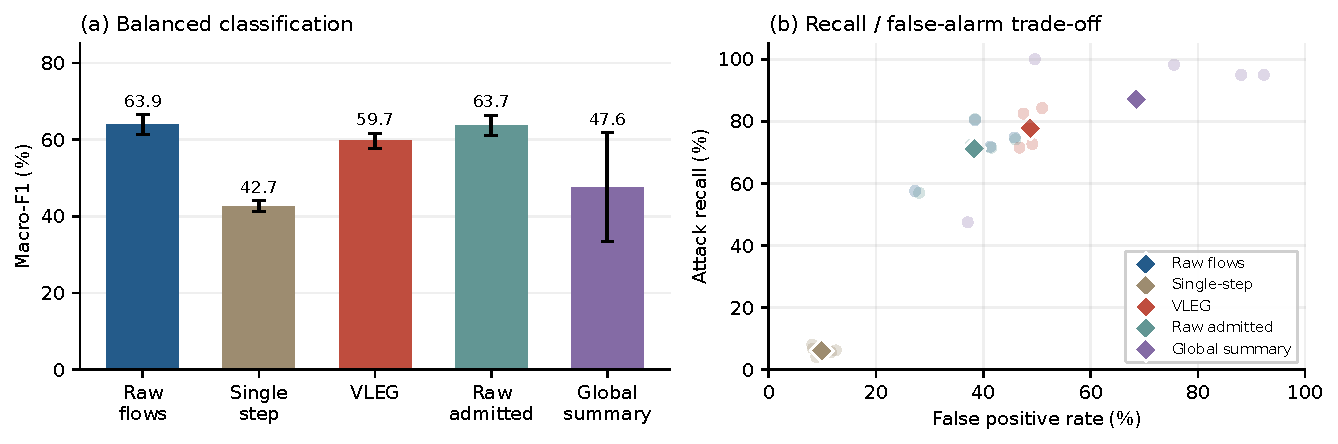
\includegraphics[width=\linewidth]{exp6_tradeoff.pdf}
\caption{Public-flow results across five memory seeds. Top: mean Macro-F1 with sample-standard-deviation bars. Bottom: attack recall versus false positive rate; faint points are individual seeds and large markers are means. The larger recall of VLEG is accompanied by more false alarms.}
\label{fig:exp6_tradeoff}
\end{figure}

Admission reaches 158/160, but 113/157 parseable accepted rules have contrary-label matches in other historical draws. This assisted screen is not a causal or human audit. There are 29 invalid first-proposal and 30 invalid VLEG predictions; they count as errors. Table~\ref{tab:exp6_cost} records construction costs; raw-on-admitted shares VLEG's cost. Fixed order/cache reuse confounds latency, and 24 identical-prompt raw/control pairs differ at temperature $0$.

\begin{table*}[!t]
\centering
\caption{Observed public-flow costs, means across five memory seeds. Construction tokens include input and output. Chat latency excludes shared retrieval and is confounded by fixed method order/cache reuse.}
\label{tab:exp6_cost}
\small
\begin{tabular}{lrrrrr}
\toprule
Condition & Construction calls & Construction tokens & Construction (s) & Query mean (s) & Query p95 (s) \\
\midrule
Raw flow retrieval & 0 & 0 & 0 & 2.12 & 2.67 \\
Unverified single-step & 32.0 & 9,405 & 126.54 & 2.23 & 2.75 \\
VLEG & 120.4 & 40,094 & 419.43 & 1.74 & 2.68 \\
Raw on admitted flows & 120.4 & 40,094 & 419.43 & 0.95 & 1.19 \\
Global summary & 1.0 & 5,947 & 23.21 & 1.21 & 1.30 \\
\bottomrule
\end{tabular}
\end{table*}

Detailed cleaning counts, provenance, per-attack results and audit procedures are supplied separately. The benchmark supports improved classification over unverified reflections, but no balanced-performance advantage over raw retrieval or production-readiness claim. Human explanation review remains incomplete.

\FloatBarrier
\subsection{Limitations}
\label{sec:limitations}
The symbolic evaluations use small populations, while the public-flow study evaluates a cleaned UNSW-NB15 testbed partition. The latter is a controlled adaptation with shared raw retrieval, not a production deployment or a complete validation of reflection-driven retrieval. Levels 1 and 2 evaluate seen combinations; Level 3 combines seen and withheld combinations. Their accuracy must not be interpreted as held-out network generalization. The flow experiment is restricted by deduplication/conflict exclusion, missing session metadata, one model and test partition, fixed method order and incomplete human explanation audits.

The synthetic rule is expressible as a single background-conditioned statement. It tests conditional rule learning, not an impossibility of global abstraction. The 7B and 70B comparisons also change model family and cannot isolate scale causally. Observed rank reversals and equal diagnostic rates are descriptive findings in these samples, not general superiority or equivalence claims.

Verification sees a known historical label and tests a candidate against one source episode. It can reject inconsistencies detected by the model, but agreement does not establish causal attribution or cross-episode validity. Reflection diagnostics based on known synthetic attributes cannot be transferred unchanged to natural traffic, where ground-truth explanations are generally unavailable.

Finally, the 7B figures are linked to the archived initial reimplementation snapshot, while updated 70B comparisons use the latest archived feedback-baseline revision. Stored item-level accuracies were independently recounted, but these historical files omit exact model digests and original verifier replies. Boolean type validation was also repaired in the oracle-audit parser; without original replies its historical impact cannot be quantified. The symbolic evaluations were not rerun, while the public-flow benchmark is independently audited against its archived predictions and frozen source. Context limits, quantization, model digests, CPU/GPU offloading and concurrent workloads require run-specific recording. The completed public-flow run records source/model/code hashes and hardware, but does not resolve every limitation of the historical experiments.

\section{Conclusions}
VLEG checks local reflections before memory admission and combines accepted reflections with source episodes during inference. In the reported symbolic experiments, refinement increases memory coverage and admitted reflections are more consistent with historical labels. Downstream benefits depend on the model and task: raw retrieval leads at 7B, while the latest archived 70B comparison gives a one-correct-evaluation pooled advantage to VLEG over raw retrieval. Hybrid grounding retains a disadvantage on some withheld combinations, and per-episode verification does not show a separate benefit for unsupported attribution.

The public-flow experiment strengthens this bounded interpretation. At 70B, VLEG improves Macro-F1 over unverified first reflections but is lower than raw retrieval, while increasing both attack recall and false alarms. High memory admission coverage therefore does not establish reliable cross-flow reasoning. Further work should test calibration and cross-episode validation on new, independently reserved data, complete explanation audits, and control timing/repeatability before making deployment claims. Historical symbolic files have now been inventoried against immutable 7B and 70B Git snapshots, and 48 stored item-level accuracy records reproduce their summaries. The latest feedback-baseline results replace stale 70B comparisons. Git provenance cannot recover missing model digests or raw verifier replies, so corrected-parser reruns and human review remain required.

\bibliographystyle{IEEEtran}
\bibliography{references}

\end{document}
